\documentclass[10pt,a4paper]{article}

\usepackage[a4paper,margin=0.72in]{geometry}
\usepackage{graphicx}
\usepackage{booktabs}
\usepackage{tabularx}
\usepackage{array}
\usepackage{enumitem}
\usepackage{microtype}
\usepackage{amsmath}
\usepackage{url}
\usepackage[colorlinks=true,linkcolor=blue,citecolor=blue,urlcolor=blue]{hyperref}
\usepackage{caption}

\setlength{\parindent}{0pt}
\setlength{\parskip}{3pt}
\setlist{nosep,leftmargin=*}
\captionsetup{font=small,labelfont=bf}
\renewcommand{\arraystretch}{1.08}

\title{Schema-Aware Text-to-SQL Generation with FLAN-T5 and Beam Reranking}
\author{Project 077 Team\\
Report prepared by Mingyuan Xu (z5707025)\\
\textit{Group members:}\\
Ruoyu Jiang (z5546234)\\
Hangji Liu (z5660625)\\
Yihan Zhou (z5676668)\\
Chenghao Ruan (z5617856)}
\date{}

\begin{document}
\maketitle

\begin{abstract}
Text-to-SQL systems translate natural-language questions into executable database queries, but they must simultaneously identify relevant schema elements and compose syntactically valid SQL. This project studies the AI4DS SQL Generator No CoT dataset using a T5-small baseline and a stronger schema-aware FLAN-T5-base system. The baseline receives the original prompt and uses greedy decoding. The final system places the question before a compact, relevance-ranked schema, canonicalises training targets, generates eight candidates, and reranks them using deterministic schema-consistency penalties. On a fixed 940-example test split, normalised exact match improves from 103/940 (10.96\%) for the baseline to 166/940 (17.66\%) for the final system. SQLGlot syntax-only validity increases from 88.19\% to 90.32\%. These gains support the value of clearer schema presentation and multi-candidate decoding, but they do not establish semantic or execution accuracy because matching populated databases are unavailable.
\end{abstract}

\textbf{Keywords:} Text-to-SQL, T5, FLAN-T5, schema linking, beam search, SQL generation

\section{Introduction}
Natural-language interfaces can make relational data accessible to users who do not know SQL. In a Text-to-SQL task, a model must map a question and a database schema to a query that selects the intended tables and columns, follows relationships, and composes filters, joins, aggregation, ordering, and nested logic. This is more demanding than ordinary text generation because a fluent-looking query may still reference the wrong identifier or express the wrong intent.

This project investigates whether a transparent sequence-to-sequence baseline can be improved by making schema information easier to use and by retaining multiple decoding alternatives. The central question is: \emph{Can schema-aware input formatting and schema-aware beam reranking improve SQL generation over a T5-small greedy baseline on a fixed held-out split?} Our contributions are (i) data inspection and reproducible preprocessing, (ii) a T5-small baseline, (iii) a schema-aware FLAN-T5-base method with beam reranking, and (iv) paired evaluation with exact-match, syntax validity, and structured error analysis.

\section{Related Work}
T5 formulates diverse NLP tasks as text-to-text generation, providing a simple encoder--decoder framework in which the prompt is the input sequence and SQL is the target sequence \cite{raffel2020t5}. FLAN-T5 extends this family with instruction tuning, which is useful when the input contains an explicit task instruction and a structured schema \cite{chung2022scaling}. Earlier Text-to-SQL systems illustrate the limitations of treating SQL as unrestricted text: Seq2SQL and SQLNet use task-specific structure to reduce invalid or poorly composed queries \cite{zhong2017seq2sql,xu2017sqlnet}, while RAT-SQL explicitly models schema relations and schema linking \cite{wang2020ratsql}. Our method is deliberately lighter-weight than a relation-aware SQL parser. It retains the T5 generation interface, but improves the representation of the schema and uses deterministic checks to select among generated candidates.

\section{Methods}
\subsection{Dataset and preprocessing}
The project uses the public AI4DS SQL Generator No CoT dataset \cite{ai4ds}. Each record contains a prompt and a response. The prompt includes task instructions, database schema DDL, a natural-language question, and sometimes a hint; the response contains the reference SQL inside a Markdown code block. Exact duplicate rows are removed before splitting, whitespace is trimmed, and the code-block markers are removed from the target.

The original dataset contains 9,399 records. Two duplicate copies are removed, leaving 9,397 unique prompt--SQL pairs. A fixed random seed of 42 is used for an 80/10/10 row-level split: 7,517 training, 940 validation, and 940 test examples. Every cleaned target begins with \texttt{SELECT}. The dataset is nevertheless challenging: 7,202 queries (76.64\%) contain a join, 1,701 contain \texttt{ORDER BY}, 1,004 contain \texttt{GROUP BY}, and 721 contain a nested query. With a 512-token T5 input limit, 690 prompts (7.34\%) are estimated to be truncated, motivating the question-first representation.

\subsection{Baseline and proposed method}
The baseline uses the pretrained \texttt{t5-small} encoder--decoder model. It receives the original cleaned prompt and generates up to 256 SQL tokens. The model is fine-tuned for ten epochs with AdamW, learning rate $5\times10^{-5}$, batch size 4, and greedy decoding (one beam). The checkpoint with the lowest validation loss is used for prediction.

The final V3 system uses \texttt{google/flan-t5-base}. It extracts the question, optional hint, and schema from the original prompt, places the question first, and linearises the schema into a compact table/column/foreign-key representation. Tables and columns with terms related to the question are ranked earlier without deleting schema elements. Training targets are conservatively canonicalised by normalising keywords and punctuation while preserving quoted literals. At inference time, Beam 8 generates eight candidates. Each candidate receives a penalty for clear schema violations, such as nonexistent tables, invalid qualified columns, unbalanced parentheses, tautological joins, and repeated decoder loops. The final candidate maximises model score minus the weighted schema penalty. V3 also uses batch size 2 with gradient accumulation 2, learning rate $10^{-4}$, weight decay 0.01, and eight epochs.

These improvements form a combined system rather than a fully controlled component ablation. Therefore, the final comparison demonstrates the effectiveness of the complete method but cannot assign the whole gain to any single change.

For integration, the repository includes a unified \texttt{src.main} entry point that exposes baseline, improvement, evaluation, \texttt{demo}, \texttt{doctor}, and test commands. The submitted notebook separately provides an offline verification path that loads aligned prediction and training artifacts, so the reported comparison does not depend on redistributing model weights or the original dataset.

\section{Experimental Setup and Metrics}
All reported results use the same fixed test split of 940 examples and aligned row order. The main metric is normalised exact match: SQL is lowercased, surrounding whitespace is removed, consecutive whitespace is collapsed, basic punctuation and comparison-operator spacing are standardised, and one trailing semicolon is ignored. This is a strict string-level diagnostic and does not prove semantic equivalence. A second metric uses SQLGlot with the SQLite dialect. A prediction is valid when it is non-empty, parses as exactly one query expression, and does not require execution or database contents.

The comparison uses the verified full-run logs and prediction artifacts recorded in the submitted notebook. Model weights are not required for the offline verification of these already-generated results.

Execution accuracy is not reported. The dataset provides prompt schemas and reference SQL but does not provide a reliable mapping from each example to a populated database instance. Executing queries against an unrelated or synthetic database would not measure the intended task.

\begin{table}[t]
\centering
\caption{Dataset characteristics and preprocessing evidence.}
\small
\begin{tabular}{lrr}
\toprule
Characteristic & Count & Percentage \\
\midrule
Raw prompt--response pairs & 9,399 & -- \\
Unique pairs after deduplication & 9,397 & -- \\
Training / validation / test & 7,517 / 940 / 940 & 80 / 10 / 10 \\
Queries containing JOIN & 7,202 & 76.64\% \\
Prompts truncated at 512 tokens & 690 & 7.34\% \\
\bottomrule
\end{tabular}
\end{table}

\section{Results}
Figure~\ref{fig:training} shows that both systems reduce training and validation loss. V3 also improves its validation task metric throughout the eight epochs, reaching 143/940 (15.21\%) at the selected final epoch. The loss values of the two models should not be compared directly because the model families and target formatting differ; they are used here to assess convergence and possible instability.

For the baseline, training loss decreases from 1.061 to 0.249 and validation loss from 0.507 to 0.231 over ten epochs. The validation loss decreases throughout the recorded run, with no rebound or visible train--validation divergence at epoch 10; the final training and validation losses are also close (0.249 and 0.231). Therefore, epoch 10 is the most evidence-supported checkpoint within the chosen ten-epoch budget and is used as the practical best checkpoint for this experiment. No epochs beyond 10 were run, so this selection is not a proof of global optimality or of the absence of later overfitting. The observed curves assess optimisation stability, but they do not by themselves establish semantic SQL correctness.

\begin{figure}[t]
\centering
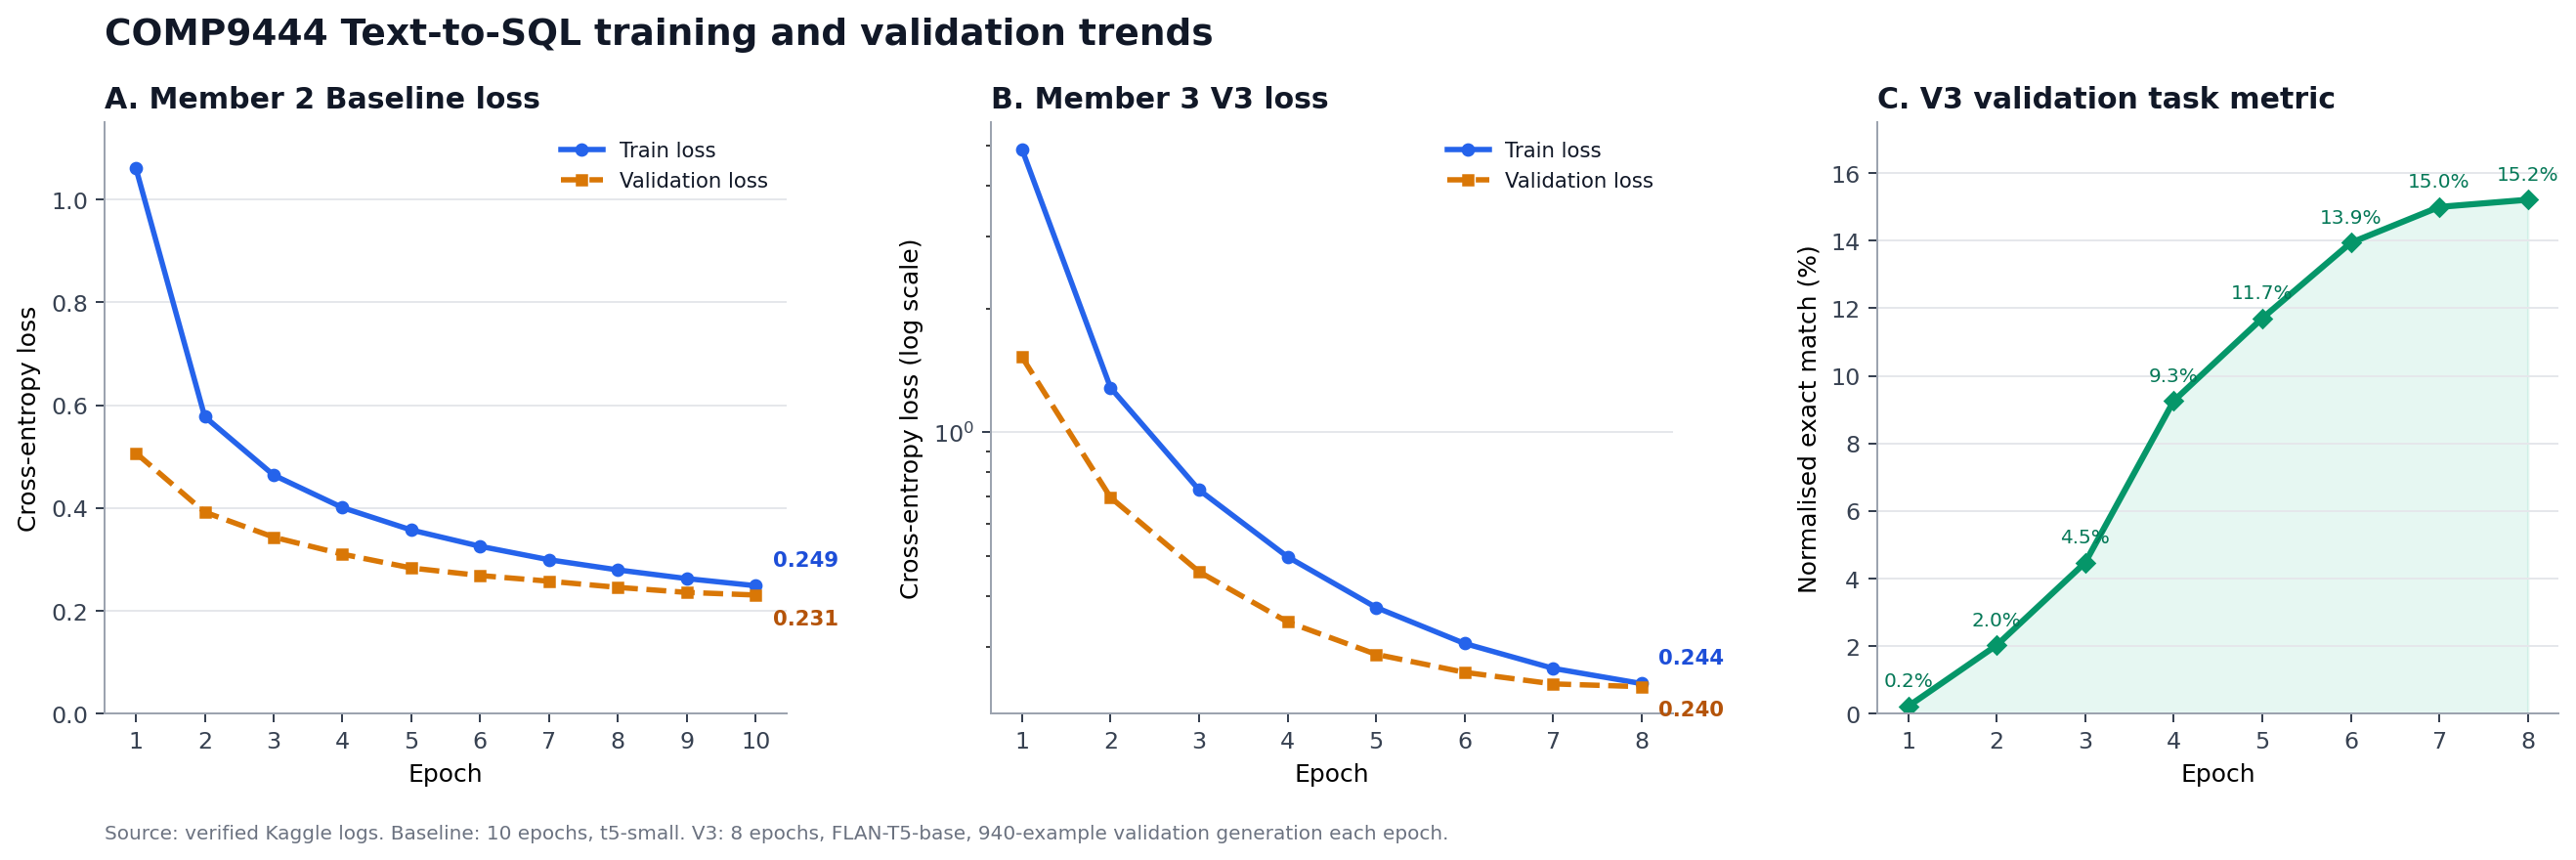
\includegraphics[width=\linewidth]{docs/experiments/figures/member3_training_trends.png}
\caption{Verified baseline and V3 training trends. The right panel reports V3 normalised exact match on the complete validation split.}
\label{fig:training}
\end{figure}

\begin{table}[t]
\centering
\caption{Final test results on 940 aligned examples.}
\small
\begin{tabular}{lrrr}
\toprule
System & Exact matches & Normalised EM & SQLGlot valid \\
\midrule
T5-small, greedy & 103 & 10.96\% & 88.19\% \\
V3, schema-aware greedy & 133 & 14.15\% & 88.94\% \\
V3, Beam 8 + reranking & 166 & 17.66\% & 90.32\% \\
\bottomrule
\end{tabular}
\end{table}

The final system improves over the baseline by 63 exact matches, or 6.70 percentage points. Within V3, Beam 8 plus reranking improves over V3 greedy by 33 examples, or 3.51 percentage points. The paired outcomes show that both systems are correct on 72 examples, V3 alone is correct on 94, the baseline alone is correct on 31, and both are wrong on 743. The validity improvement is smaller than the exact-match improvement, which is expected: a query can be syntactically parseable while selecting the wrong table, column, join, filter, or aggregation.

Qualitative inspection identifies five recurring error types: schema-linking errors, incorrect join keys or aliases, wrong query intent, incomplete nested or compositional structure, and surface-form differences that may still be semantically equivalent. These observations explain why a syntax metric is substantially higher than exact match and motivate execution-based evaluation in future work.

One representative error distinguishes syntactic plausibility from semantic correctness: a prediction used \texttt{COUNT(category\_id)} where the reference required \texttt{COUNT(DISTINCT category\_id)}. Both forms can parse successfully, but they return different answers when a category appears more than once. This example supports reporting SQL validity alongside exact match rather than treating validity as task success.

Published text-to-SQL systems are not directly comparable here because they commonly use different datasets, schema splits, database engines, and evaluation protocols. We therefore use the reproduced baseline as the controlled comparator rather than claiming an external state-of-the-art ranking.

\section{Discussion}
The main strength of the proposed system is that it improves the information presented to the model without requiring a new SQL grammar or a database execution loop. Question-first ordering protects the user request when the input is truncated, relevance ranking exposes likely identifiers earlier, and beam reranking can reject candidates with clear schema violations. The fixed split, aligned prediction artifacts, and explicit metric definitions also make the comparison reproducible offline.

There are four important limitations. First, normalised exact match is still a string metric: it can reject equivalent queries and can reward a reference-specific surface form. Second, SQLGlot validity checks syntax and basic query structure, not execution results, schema semantics, or answer correctness. Third, the row-level split is not schema-disjoint, so related schemas may occur across training and test sets. Fourth, V3 changes model capacity, prompt format, target normalisation, checkpoint selection, and decoding together. Controlled ablations are needed to isolate their individual effects. Finally, most examples remain incorrect under exact match, so the system is not ready to be described as a reliable production SQL interface.

The most important next step is to recover the correct populated database and example-to-database mapping, then report execution accuracy on both reference and predicted SQL. Other useful directions include schema-disjoint evaluation, statistical significance tests, component-wise ablations, stronger schema linking, constrained decoding, and semantic equivalence metrics.

\section{Conclusion}
This project built a reproducible Text-to-SQL pipeline from dataset cleaning through model training, decoding, and evaluation. The dataset analysis showed that long schema-rich prompts and frequent joins make the task challenging. On the fixed 940-example test split, the T5-small greedy baseline achieved 10.96\% normalised exact match, while the schema-aware FLAN-T5-base system with Beam 8 and schema reranking achieved 17.66\%. SQLGlot syntax-only validity increased from 88.19\% to 90.32\%. The results support clearer schema presentation and multi-candidate decoding, but they do not establish semantic or execution accuracy. The conclusions are therefore evidence of improved string-level and syntax-level performance, not proof that the generated SQL always returns the correct answer.

\begin{thebibliography}{9}
\bibitem{raffel2020t5}
C. Raffel et al., ``Exploring the Limits of Transfer Learning with a Unified Text-to-Text Transformer,'' \emph{JMLR}, vol. 21, no. 140, 2020. Available: \url{https://arxiv.org/abs/1910.10683}

\bibitem{chung2022scaling}
H. W. Chung et al., ``Scaling Instruction-Finetuned Language Models,'' \emph{JMLR}, vol. 25, 2024. Available: \url{https://arxiv.org/abs/2210.11416}

\bibitem{zhong2017seq2sql}
V. Zhong, C. Xiong, and R. Socher, ``Seq2SQL: Generating Structured Queries from Natural Language using Reinforcement Learning,'' EMNLP, 2017. Available: \url{https://arxiv.org/abs/1709.00103}

\bibitem{xu2017sqlnet}
X. Xu, C. Liu, and D. Song, ``SQLNet: Generating Structured Queries from Natural Language without Reinforcement Learning,'' arXiv:1711.04436, 2017. Available: \url{https://arxiv.org/abs/1711.04436}

\bibitem{wang2020ratsql}
B. Wang et al., ``RAT-SQL: Relation-Aware Schema Encoding and Linking for Text-to-SQL Parsers,'' ACL, 2020. Available: \url{https://arxiv.org/abs/1911.04942}

\bibitem{ai4ds}
AI4DS, ``SQL Generator No CoT,'' Hugging Face Datasets. [Online]. Available: \url{https://huggingface.co/datasets/AI4DS/sql_generator_no_cot}

\end{thebibliography}

\end{document}
